%2.3_2 プログラムとスクリプト

\clearpage
\subsection{プログラムとスクリプト}

プログラムを打ち込むためには、「HSPスクリプトエディタ」というツールを使うことを覚えました。
このエディタに打ち込む言葉のことを「スクリプト」と呼んでいることを覚えていますか?
スクリプトは、プログラムがどのように動くかを書いた設計図のようなものです。これは、ソースコードとも呼ばれています。
皆さんが使っているアプリやゲーム、パソコンのプログラムもソースコードをもとにして作られています。
スクリプトエディタは、スクリプトを書いて実行するためのツールです。
\vskip\baselineskip
スクリプトは、プログラムを作るための元になるものですが、その書き方には色々な種類があります。
これは英語とも日本語とも違う特別なルールを持った言葉です。この言葉は「プログラム言語」と呼ばれていて、やりたいことに合わせて色々な種類があります。

\begin{figure}[H]
    \begin{center}
        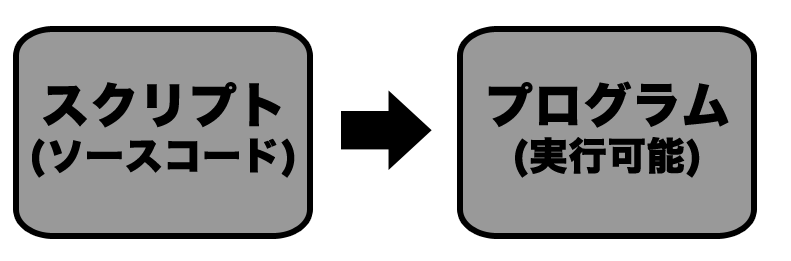
\includegraphics[keepaspectratio,width=11.509cm,height=3.803cm]{text02-img/text02-img022.png}
    \end{center}
\end{figure}

今回、皆さんが使うHSPは小文字のアルファベット(英語)でスクリプトを打ち込みます。でも英語を知らなくても構いません。漢字変換がいらないので、慣れれば英語の方が打ち込むのが早くなりますし、世界中の人が同じ方法で打ち込んでいるので、今覚えておけば将来にも役立つはずです。

